\documentclass[11pt, a4paper]{article}
\usepackage{graphicx} % Required for inserting images
\usepackage{listings}
\usepackage{color}
\usepackage{hyperref}
\usepackage{url}

\title{A Web Based Command Line Interface for Specifying Multiway Dataflow Constraint Systems}
\author{Bo Aanes}
\date{June 2023}
\lstset{
    frame=single,
    basicstyle=\linespread{0.8}\footnotesize\ttfamily,
    keywordstyle=\color{red},
    numbers=left,
    numbersep=5pt,
    showstringspaces=false, 
    stringstyle=\color{blue},
    commentstyle=\color{gray},
    breakatwhitespace=true,
    breaklines=true,
    postbreak=\mbox{\textcolor{violet}{$\hookrightarrow$}\space},
    tabsize=4,
}

\begin{document}

\begin{titlepage}
    \centering
    \vspace*{\fill}
    {\huge\bfseries A Web Based Command Line Interface for Specifying Multiway Dataflow Constraint Systems\par}
    \vspace{2cm}
    {\Large\itshape Bo Victor Isak Aanes\par}
    \vfill
    {\LARGE INF319 Project\par}
    {\cshape\large Department of Informatics\par}
    {\scshape\large University of Bergen\par}
    {\scshape\large Norway\par}
    \vspace{1cm}
    {\large \today\par}
    \vfill
\end{titlepage}
\tableofcontents
\clearpage

\section{Introduction}
\label{sec:introduction}
Graphical user interfaces (GUIs) are prevalent in most of today's technology that involves user interaction. However, developing and maintaining GUIs can still be difficult. Much of this is because as a GUI involves a larger set of state, the business logic neede in order to keep track of this state quickly becomes complex. This problem grows even bigger when we introduce dependencies between elements of the GUI. Multiway dataflow constraint systems (MDCS) is a programming model designed to let a developer specify dependencies between elements of the GUI using constraints \cite{semantics}. This is usually done declaratively and MDCS will handle all business logic related to these constraints. 

\section{Background}
\label{sec:background}
\subsection{Multiway Dataflow Constraint Systems}
\label{sec:mdcs}
A multiway dataflow constraint system consists of a set of variables and a set of constraints. A variable holds a value which can be modified, and a constraint consists of a set of methods which contain expressions that can modify a variable.

Libraries that implement MDCSs usually also handles enforcing of constraints, such that whenever a value gets updated by a user the constraint system automatically satisfies all its constraints. The main part of \textit{solving} a constraint system is achieved through what is called \textit{planning} \cite{planners}. When a variable is updated by a user, the constraints involving this variable may no longer be satisfied, that is, that the relations specified in the methods no longer hold. As such, we have to select the appropriate methods to invoke in order to enforce the given constraints, such that the constraint system is satisfied. This is what the planner does.

When a user updates a variable, they will expect that the constraint system does not overwrite that variable instantly. Because of this we do not want the planner to select a method writing to this variable, but rather a method that reads from it. I.e., we want to select the methods from the constraints that result in the least surprising outcome to the user. This is what is known as a \textit{hierarchical} planning algorithm \cite{planners}.

The hierarchical planner assigns a strength to each variable, which gets updated when a user modifies a variable. The variable with the highest strength is the one that was updated most recently, and the variable with the lowest strength was the one updated least recently. By assigning a strength to the variables, the planner can make selections on which variables to preserve by selecting the appropriate methods.

When the appropriate methods are selected, they are invoked in the topological order of the dataflow graph. This is done to ensure that all variables are updated in the correct order, such that no variable is updated before its dependencies are updated.

\subsection{HotDrink}
\label{sec:hotdrink}
HotDrink is a JavaScript library for specifying multiway dataflow constraint systems \cite{hotdrink}. It provides both an API and a DSL for this purpose. Variables can be declared along with constraints between these, which in turn can be bound to specific HTML-elements. The constraints themselves contain \textit{methods} which can hold expressions or JavaScript functions that return values which are written to specified variables. In Listing \ref{lst:currencyhotdrink}, we can see how we can use HotDrink's API and DSL to define a constraint system to perform currency conversion between EUR and NOK.

\begin{lstlisting}[language=java, caption={Currency conversion in HotDrink.}, label={lst:currencyhotdrink}]
const constraintSystem = new ConstraintSystem();

const component = component`
    var exchangeRate = 10;
    var eur = 0;
    var nok = 0;

    constraint {
        eurToNok(eur, exchangeRate -> nok) = eur * exchangeRate;
        nokToEur(nok, exchangeRate -> eur) = nok / exchangeRate;
    }
`;

constraintSystem.addComponent(component);
constraintSystem.update();
\end{lstlisting}

We first define a constraint system using the \texttt{ConstraintSystem} class. We then define a component using the \texttt{component} template literal, which contains specifications for a currency conversion using HotDrink's DSL. Here we define variables and a constraint containing two methods: one for converting EUR to NOK, and one for converting NOK to EUR. After specifying our component, we add this component to the constraint system and call \texttt{constraintSystem.update()} to enforce the constraint.

The variables defined in the constraint system in Listing \ref{lst:currencyhotdrink} can be bound to elements in the document object model (DOM), e.g., two input fields. When the user changes one of these input fields, the other one's value will be updated to the correct value determined by the constraint system.

\subsection{Structure Manipulation}
\label{sec:structuremanipulation}
\textit{WarmDrink} is a domain specific language (DSL) for defining relation between components in constraint systems \cite{warmdrink}. This allows for defining what we call \textit{intercalating constraints} which can manipulate values between elements in structures such as lists or trees. An example of this could be a multi-city flight itinerary \cite{warmdrink}. Let us say the first flight is at 15th of June, then the next flight can be no earlier than 15th of June as well. This relation can be introduced as an intercalating constraint between all flights in flight itinerary. The date of each flight must be equal to or greater than the preceding flight's date. If one of the flight's date gets updated, then so must all the succeeding flights as well.

\subsection{React}
\label{sec:react}
React is a JavaScript library for building user interfaces \cite{react}. It is based on the concept of components, which are reusable pieces of code that can be composed together to build complex user interfaces. React components are written in JavaScript, and can be written using either a class-based or a functional approach. In Listing \ref{lst:reactcomponent}, we can see an example of a React component written using the functional approach. Notice how the \texttt{return}-function contains HTML-like syntax. This is known as JSX (or JavaScript XML), which is an extension of JavaScript's syntax that allows for using HTML directly in you JavaScript files. React then transpiles the code into regular JavaScript, which can be run in a web browser.

\begin{lstlisting}[language=java, caption={A React component written using the functional approach.}, label={lst:reactcomponent}]
function MyComponent(props) {
    return (
        <div>
            <h1>{props.title}</h1>
            <p>{props.text}</p>
        </div>
    );
}
\end{lstlisting}

React components can be rendered to the DOM using the \texttt{ReactDOM.render} method. This method takes a React component and a DOM element as arguments, and renders the component to the DOM element. In Listing \ref{lst:reactrender}, we can see how we can render the component from Listing \ref{lst:reactcomponent} to the DOM. Notice how we pass \textit{props} from the parent component down to the child component within the JSX.

\begin{lstlisting}[language=java, caption={Rendering a React component to the DOM.}, label={lst:reactrender}]
ReactDOM.render(
    <MyComponent title="Hello, world!" text="This is my first React component." />,
    document.getElementById('root')
);
\end{lstlisting}

\subsection{Web Application Programming Interfaces}
\label{sec:apis}
An application programming interface (API) is a set of rules and protocols for building software applications. It defines how different software components can interact with each other. This can for example be between a frontend web application and a backend database. This is known as a Web API, or an HTTP API.

A web server can provide \textit{endpoints} for a client to send requests to. These endpoints are URLs that the client can send HTTP requests to, and the server will respond with a HTTP response. The client can send different types of requests, such as GET, POST, PUT, and DELETE. These requests are used to retrieve, create, update, and delete data from the server, respectively. The server can then respond with different types of responses, such as 200 OK, 201 Created, 400 Bad Request, and 404 Not Found. These responses are used to indicate whether the request was successful or not, and can also contain data.

\subsection{Haskell}
\label{sec:haskell}
Haskell is a purely functional programming language first released in 1990 \cite{haskell}. It is a statically typed general purpose language which uses lazy evaluation and type inference. Lazy evaluation is a technique where the compiler does not evaluate expressions until they are needed. And type inference is a feature in the compiler which can infer the types of expressions without them having to be explicitly annotated in the actual code..

Haskell also provide a powerful type system, which allows for the creation of custom types and type classes. Type classes are similar to interfaces in object-oriented programming languages, and can be used to define functions that can be used on different types. For example, the \texttt{Show} type class defines a function \texttt{show} which can be used to convert a value to a string. While the \texttt{Eq} type class is used for determining equality between values.

Data types in Haskell can be considered algebraic data types. They can be either \textit{product types} or \textit{sum types}. Product types are types that contain multiple values, such as tuples and records. Sum types are types that can be one of multiple types, such as the \texttt{Maybe} type. The \texttt{Maybe} type can either be \texttt{Just a} or \texttt{Nothing}, where \texttt{a} is a type variable. This type is used to represent values that may or may not be present, such as the result of a database query.

\newpage

\section{Frontend Implementation}
\label{sec:frontend}

\subsection{Component View and State}
\label{sec:componentview}
The frontend part of our CLI tool is written in TypeScript \cite{typescript} with React as our frontend library of choice.The main component \texttt{App} is the root component of our frontend and embodies everyhting the user sees and interacts with. The user is presented with a split screen consisting of a two main components: the view of the constraint system, and the terminal, see Figure \ref{fig:view}.

\begin{figure}[h]
    \centering
    \makebox[\textwidth][c]{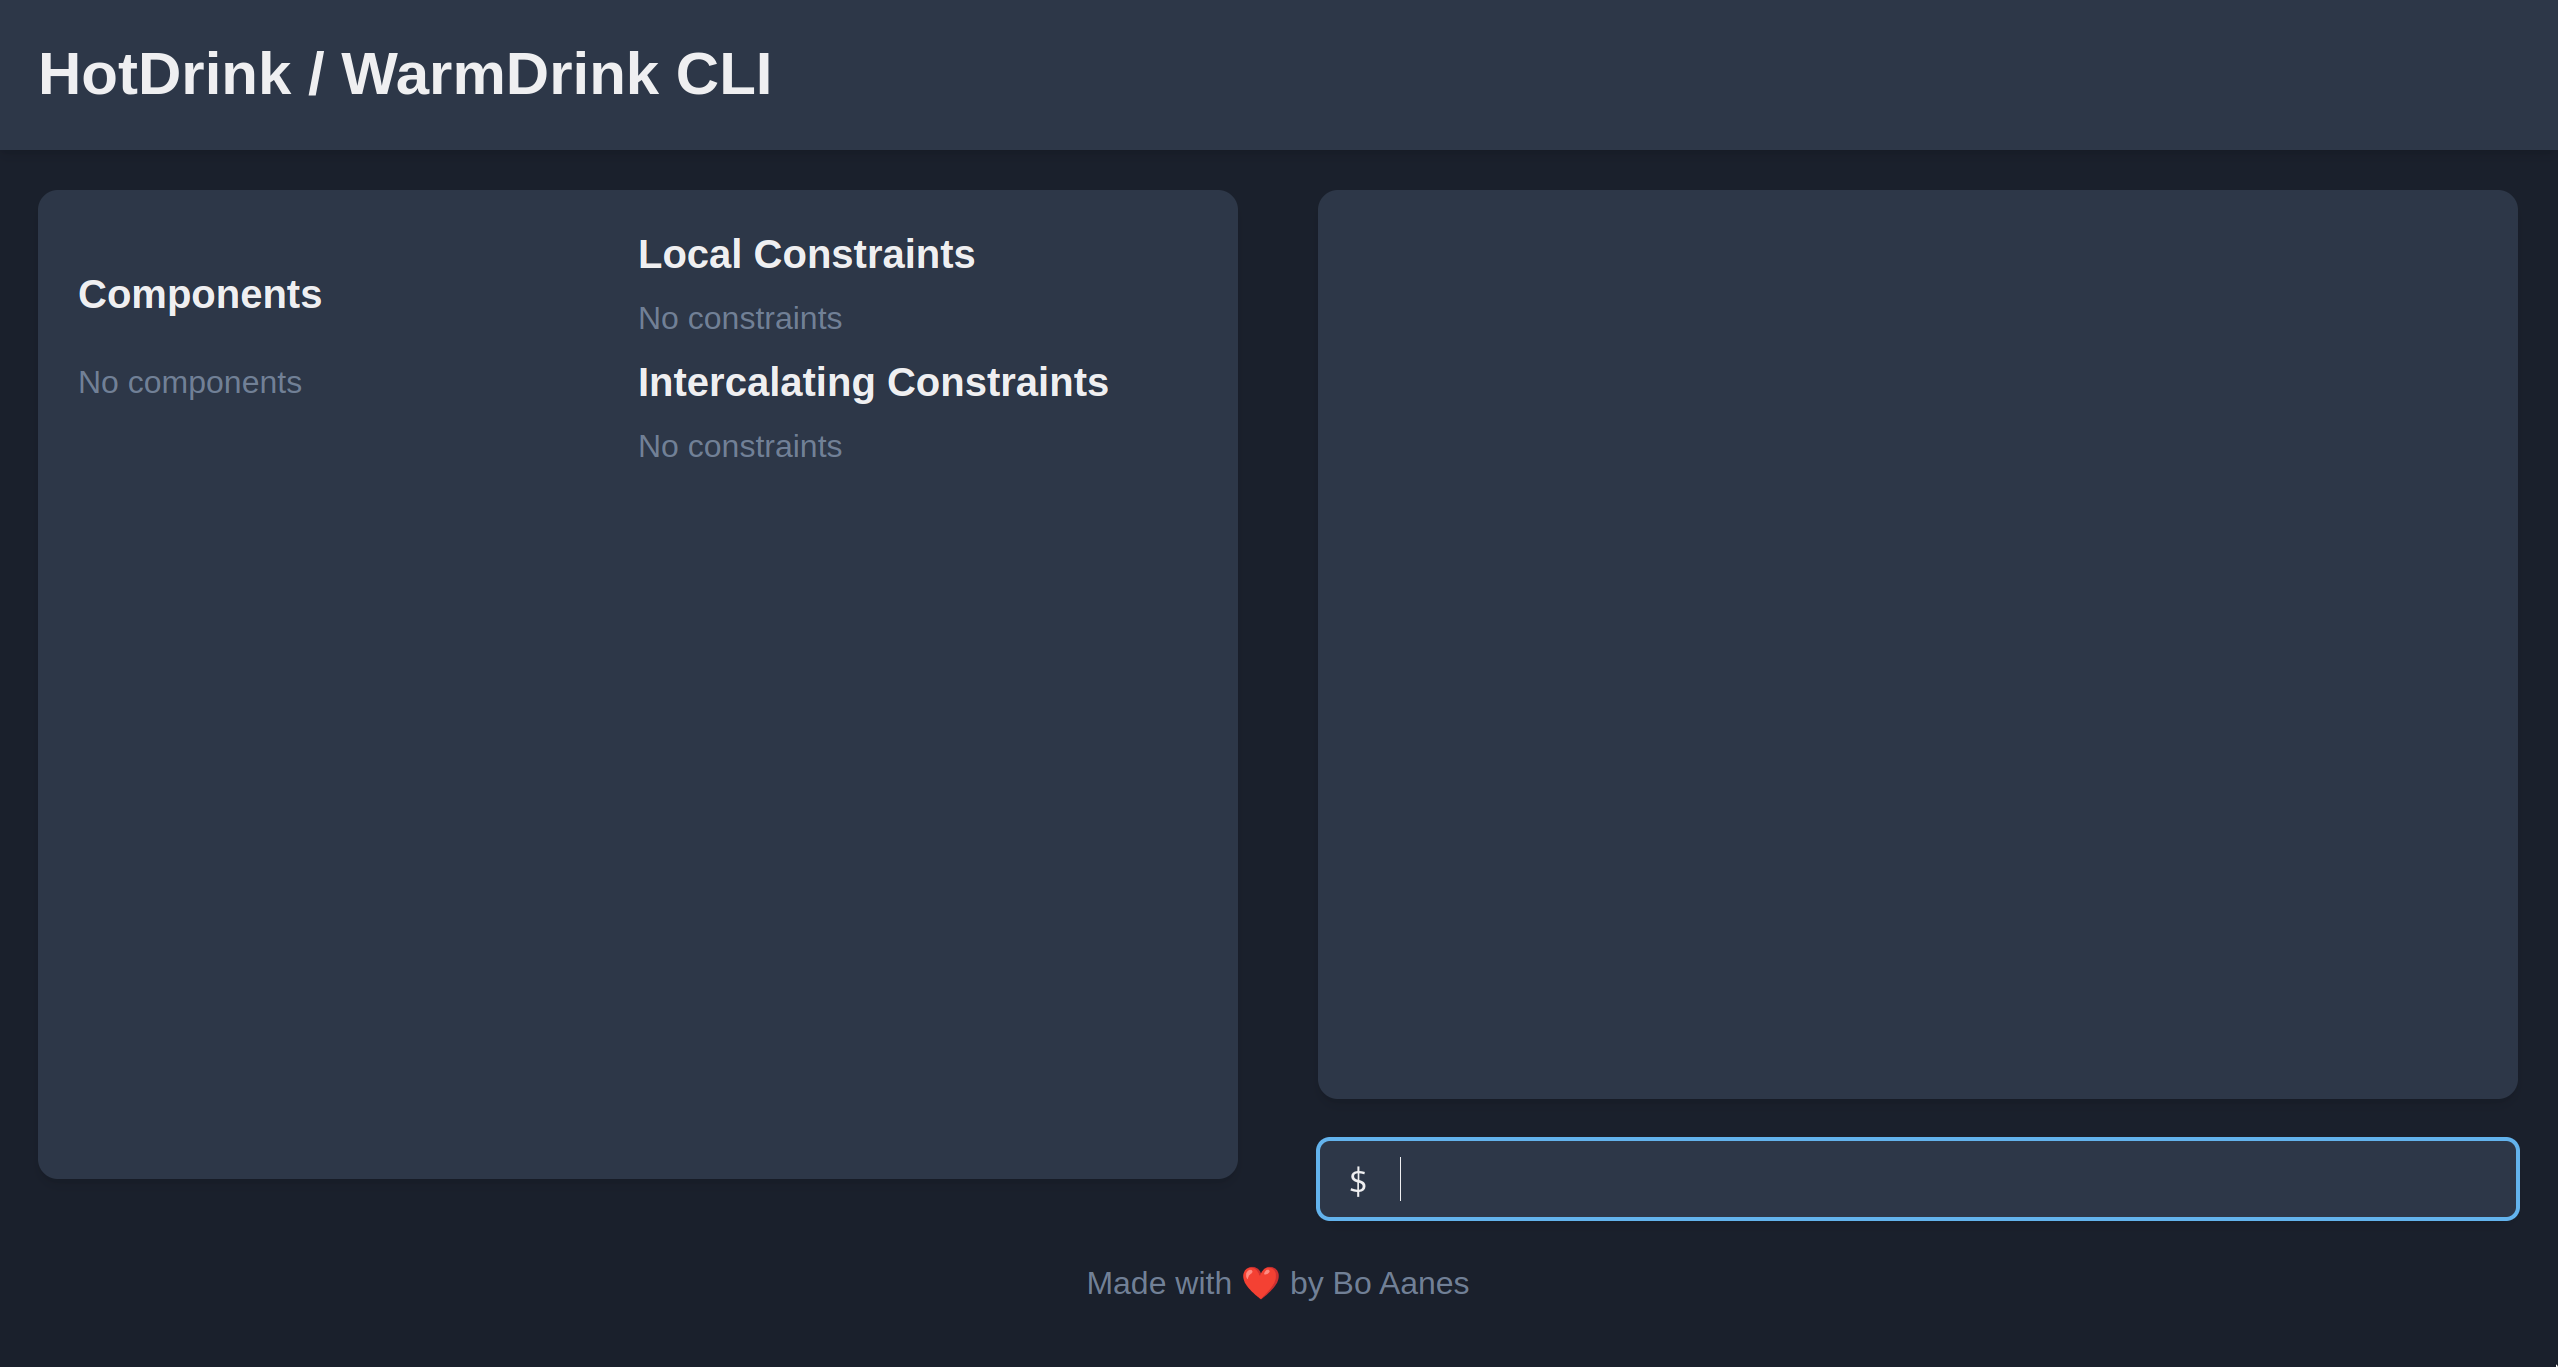
\includegraphics[width=1.2\textwidth]{figures/view.png}}
    \caption{The view of the constraint system and the terminal.}
    \label{fig:view}
\end{figure}

In addition to the view of the program, the \texttt{App}-component also manages the state of the constraint system. We have defined types for components, constraints, methods, variables and component lists as can be seen in Listing \ref{lst:types}.

\begin{lstlisting}[float, language=java, caption={Types for constraint systems.}, label={lst:types}]
export interface Method {
  methodName: string;
  inputs: string[];
  expressions: Array<[string, string | undefined]>;
}

export interface Constraint {
  constraintName: string;
  methods: Method[];
}

export interface Variable {
  varID: string;
  varValue: number | boolean;
}

export interface IComponent {
  compID: number;
  variables: Variable[];
  strength: string[];
}

export interface ComponentList {
  components: IComponent[];
}
\end{lstlisting}

To manage state in React we use a \textit{hook} \cite{reacthooks} called \texttt{useState}. \texttt{useState} is a function that takes an optional default value state and returns an array consisting of two elements. The first being the current state, and the second begin a function to update the state. In Listing \ref{lst:usestate}, we show how the state for the application is handled in the root component. We manage state for the components, the local constraints, as well as the intercalating constraints. In addition to this, we also have a state \texttt{highlighted}, and a state \texttt{enforceFromIndex}. \texttt{highlighted} contains a list of strings indicating elements in the GUI that are highlighted in a unique color, this is explained later in this Section. \texttt{enforceFromIndex} indicates the index of the component where the enforcing of constraints should be triggered. E.g., if a user updates a value in \texttt{component 2}, then this is where the constraints should be enforced from, as no values needs to be changed in the preceding components in order to satisfy the entire constraint system.

\begin{lstlisting}[float, language=java, caption={Using \texttt{useState} to manage state.}, label={lst:usestate}]
const [components, setComponents] = useState<IComponent[]>([]);
const [constraints, setConstraints] = useState<Constraint[]>([]);
const [intercalatingConstraints, setIntercalatingConstraints] = useState<
  Constraint[]
>([]);
const [highlighted, setHighlighted] = useState<string[]>([]);
const [enforceFromIndex, setEnforceFromIndex] = useState<number>(0);
\end{lstlisting}

\subsection{Terminal and User Interaction}
\label{sec:terminal}

For the terminal emulator of our frontend implementation we have put together two visual components: one box where the user can see their command history, as well as an input field at the bottom (see Figure \ref{fig:view}). While this is actually just a simple form with a display of everything previously entered into the input field, the idea is that it should still feel like a regular terminal emulator. The \texttt{Terminal} component contains two main states: one for the current state of the input field, as well as one for the command history. In addition to these states, we have a function \texttt{submit}, which takes a \textit{FormEvent} as input and handles this input as a command. This is our main function for the business logic of our CLI, it handles all commands and is responsible for all user interaction.

The function \texttt{submit} is triggered when the form containing the input field is submitted. We use HTMLs native \texttt{onSubmit} event handler to trigger this function, like so:

\begin{verbatim}
<form onSubmit={submit}>
\end{verbatim}

The function then prevents the default behavior of the form, which is to reload the page, and instead uses the current state of the input field as a command. The input state is then split into words, where the first word is treated as the command, and the following words are treated as arguments. First we check if the command is a valid command. If it is not a valid command, we clear the input state and append a message "Invalid command" to the command history and return void. Proceeding, we have a \textit{switch} statements with cases that match the individual commands, where each case handles the business logic related to that command. This may be to insert a new component, swap the positions of two components, adding or updating a variable, or highlighting a given variable or constraint. Figure \ref{fig:example} shows an example state of the application where the user has defined some components with variables and constraints and highlighted both a variable, a method, and a constraint. Notice how the components and constraints are displayed, as well as the command history on the right side.

\begin{figure}[h]
    \centering
    \makebox[\textwidth][c]{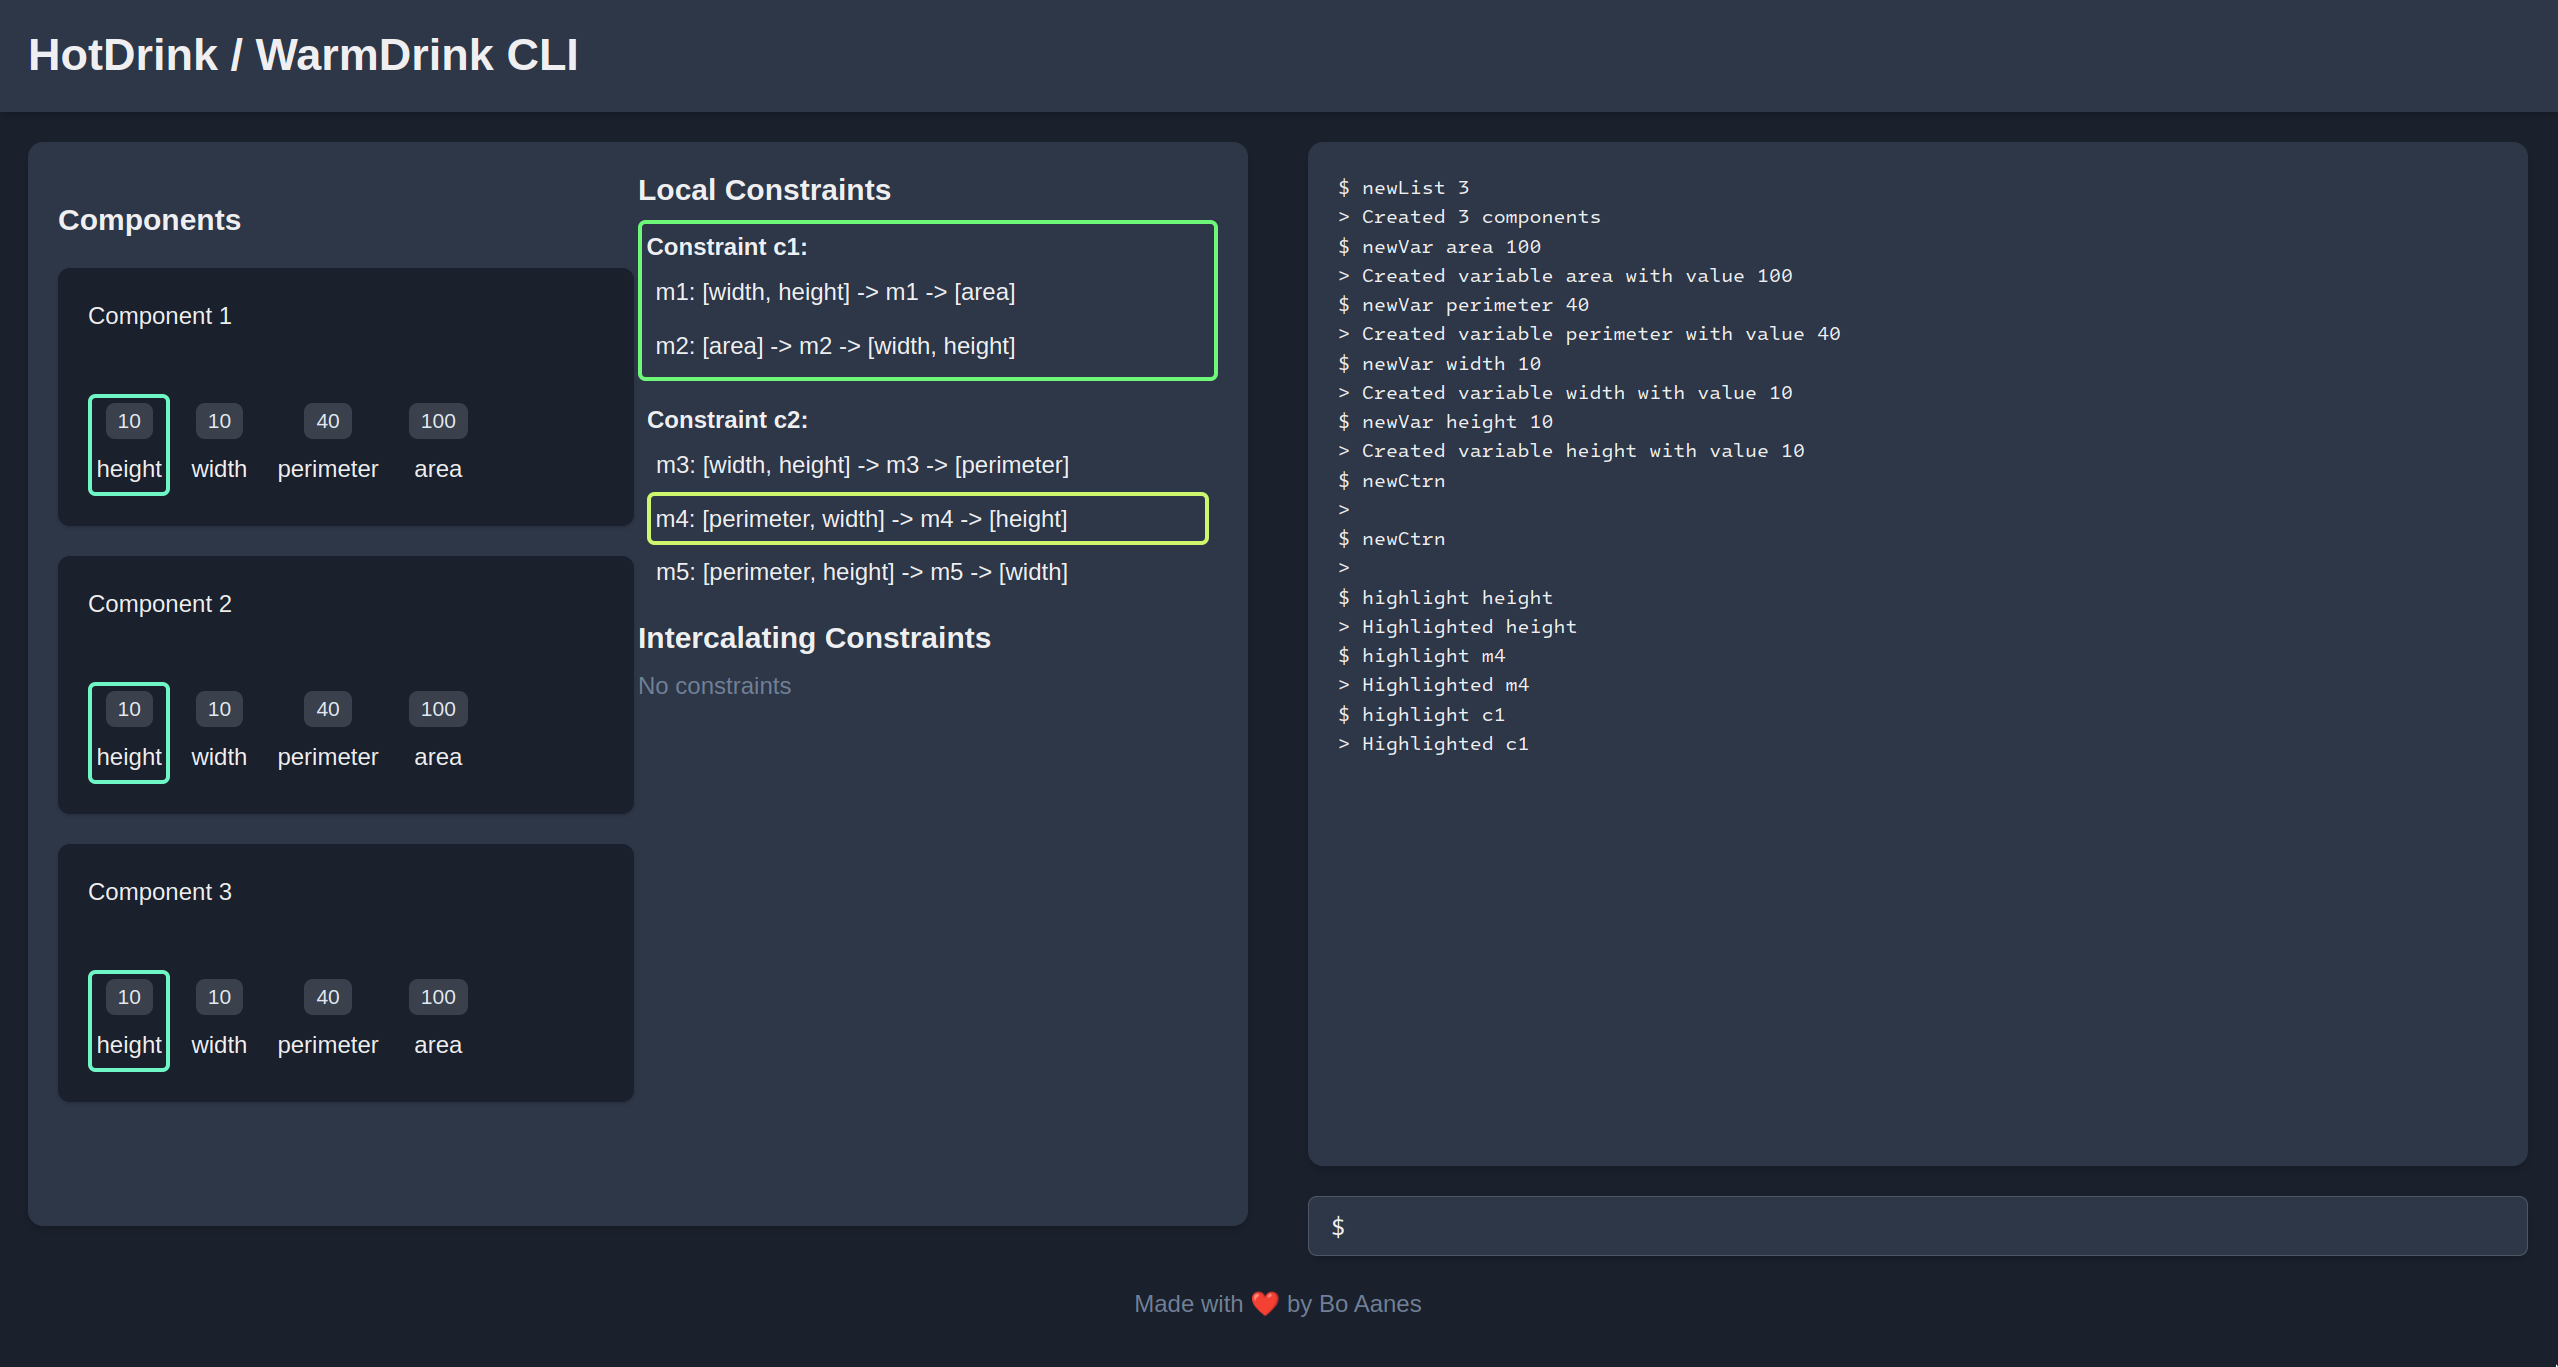
\includegraphics[width=1.2\textwidth]{figures/example.png}}
    \caption{Example state of the application with some highlighted elements.}
    \label{fig:example}
\end{figure}

\section{API Implementation}
\label{sec:api}
\subsection{Haskell API}
\label{sec:haskellapi}
To handle the algorithmic parts, mainly planning and solving of the constraint system, we have built an API in Haskell using a library called \textit{Scotty} \cite{scottyArticle, scottyHackage}. Scotty provides a minimal way of defining endpoints for HTTP requests. In Listing \ref{lst:scottyExample} we can see how a simple endpoint for a GET-request reponding with "Hello World" can be created. The function \texttt{main} calls the function \texttt{scotty} with two arguments, a port number for where to listen for requests, as well as a \texttt{ScottyM ()}\footnote{\url{https://hackage.haskell.org/package/scotty-0.12.1/docs/Web-Scotty.html\#t:ScottyM}}. The \texttt{ScottyM ()} is scotty's own monad for performing sequential operations. Within the outermost do-notation in Listing \ref{lst:scottyExample} we can list endpoints with their respective HTTP request types. In the example, we use the function \texttt{get} which takes two arguments, a route pattern ("/hello") and a \texttt{ActionM ()}. The \texttt{ActionM ()} is an action we want the server to perform, in this case return a raw text displaying "Hello World!".

\begin{lstlisting}[language=haskell, caption={Example of a simple endpoint in Scotty.}, label={lst:scottyExample}]
main = scotty 3000 $ do
  get "/hello" $ do
    text "Hello World!"
\end{lstlisting}

As stated previously, we use our API to handle the algorithmic parts of the constraint system. The main idea here, is to use our Haskell API as a black box. We send a request to the server with our current state of the constraint system, and the server responds with our updated variable values, which we assign to our frontend state. Becuase of this, we need to be able to accept requests with a body that contains our state. HTTP requests can carry this information structured as JSON\footnote{\url{https://www.json.org/json-en.html}}, but because Haskell is statically typed, we need to define data types for how this JSON-data is structured, along with parsers and encoders.

To achieve this we use a library called \textit{Aeson} \cite{aeson}. Aeson provides a way to encode and decode Haskell data types to and from JSON. In Listing \ref{lst:aesonExample} we show an example of how we can define a data type \texttt{JSONVariable} with two fields, \texttt{varID} and \texttt{varValue}.

\begin{lstlisting}[float, language=haskell, caption={Example of a data type for a JSON-variable.}, label={lst:aesonExample}]
{-# LANGUAGE DeriveAnyClass    #-}
{-# LANGUAGE DeriveGeneric     #-}

data JSONVariable
  = JSONVariable
      { varID :: String
      , varValue :: String
      }
  deriving (FromJSON, Generic, ToJSON)
\end{lstlisting}

The language extensions \texttt{DeriveAnyClass} and \texttt{DeriveGeneric} are used to derive the \texttt{FromJSON} and \texttt{ToJSON} type classes. These type classes are derived automatically, which provide a parser and encoder without having to write these manually.

Furthermore, we have defined data type for the API's input and output JSON types. As stated earler, the API recieves the state of the whole constraint system, and solves this before outputing the new values of each variable. Listing \ref{lst:IOtypes} shows how these data types are defined.

\begin{lstlisting}[language=haskell, caption={Input and output data types for the API.}, label={lst:IOtypes}]
data Input
  = Input
      { components               :: [JSONComponent]
      , constraints              :: [JSONConstraint]
      , intercalatingConstraints :: [JSONConstraint]
      , enforceFromIndex         :: Int
      }
  deriving (FromJSON, Generic, ToJSON)

data Output where
  Output :: {vars :: Map String [JSONVariable]} -> Output
  deriving (FromJSON, Generic, ToJSON)
\end{lstlisting}

The \texttt{Input} data type contains the set of components, constraints, and intercalatingConstraints, in addition to the index of which component to enforce constraints from, as described in the state of the frontend application from Section \ref{sec:componentview} and Listing \ref{lst:usestate}. The \texttt{Output} data type is a map from component identifiers to values of JSONVariables.

\begin{lstlisting}[language=haskell, caption={Example of an endpoint for the API.}, label={lst:endpoint}]
routes :: ScottyM ()
routes = do
  post "/" $ do
    input <- jsonData :: ActionM Input
    let componentList = solve input
    case satisfied of
      Just newVars -> do
        json $ Output newVars
      Nothing -> do
        status status500
\end{lstlisting}

With these defined data types we can now use functions for capturing the JSON request body as well as respond with a JSON response of the desired structure. In Listing \ref{lst:endpoint}, we decode the JSON request body using the function \texttt{jsonData}, we then solve the constraint system using a MDCS library in Haskell, before returning the formatted response with \texttt{json}. In the case that there is an error in solving the constraint system, we return a HTTP 500 response, which indicates an internal server error. This is a simplified version of the actual function in our implementation, but provides an overview of how we handle requests and responses.

\subsection{Sending Requests and Receiving Responses}
\label{sec:requests}

When one of the states regarding components, constraints, or intercalating constraints changes (which we discussed in Section \ref{sec:componentview} and outlined in \ref{lst:usestate}), the constraint system may be un-satisfied. Things that could lead to this can be e.g., the user updating a variables value, introducing a new constraint or simply inserting a new component, among other operations. When a state changes in React, we can use the \textit{useEffect}-hook\footnote{\url{https://react.dev/reference/react/useEffect}} to trigger side-effects. The useEffect-hook is a function that takes another function as input (the effects we would like to perform), as well as a dependency array --- an array containing the states which when changed, should trigger the effects. Listing \ref{lst:useeffect} outlines how we utilize the useEffect-hook to send a request to the Haskell API and update the state using the response.

\begin{lstlisting}[language=java, caption={useEffect-hook to send a request to the Haskell API and update the state.}, label={lst:useeffect}]
useEffect(() => {
  const enforceConstraints = async () => {
    const response = await fetch('http://localhost:8000/', {
      method: 'POST',
      headers: {
        'Content-Type': 'application/json'
      },
      body: JSON.stringify({
        components: components,
        constraints: constraints,
        intercalatingConstraints: intercalatingConstraints,
        enforceFromIndex: enforceFromIndex
      });
    });
    const data = await response.json();
    setComponents(data);
  }
  enforceConstraints();
}, [components, constraints, intercalatingConstraints, enforceFromIndex]);
\end{lstlisting}

As with the function outline in Listing \ref{lst:endpoint}, the function outlined in Listing \ref{lst:useeffect} is a simplified version of the actual implementation. The actual implementation uses a helper function for the request to the server, which restructures the state to fit the data types defined in Haskell. In addition to this, the actual implementation contains error handling, as well as a check to see if the response is different from the current state, before updating the state. This is to avoid an infinite loop of requests and responses. The call to \texttt{setComponents} is also simplified in the example, as \texttt{data} is not in its correct format, but still illustrates the functionality of setting the new state of components.

\section{Usage}
\label{sec:usage}
The user can interact with the application entirely throught the terminal. The terminal has a set of commands that can be listed with the \texttt{help}-command. Listing \ref{lst:help} shows the available commands.

\begin{lstlisting}[caption={Available commands in the terminal.}, label={lst:help}]
$ help
> Available commands:
> newComp - Add a new component
> newList <n> - Add a new list of size n
> newVar <varID> <value> - Add a new variable to all components
> newCtrn - Add a new constraint to all components
> newIctrn - Add a new intercalating constraint
> updVar <compID> <varID> <value> - Update the given variable
> delVar <varID> - Delete the given variable
> insAfter <compID> - Insert a new component after the given component
> swap <compID> <compID> - Swap the given components
> rmv <compID> - Remove the given component
> highlight <identifier> - Highlight the element for the given identifier
> reset - Reset highlights
> help - Display this help message
\end{lstlisting}

Most of these commands are self explanatory, as they manipulate the constraint system in a rather simple way. However some are worth elaborating further on, mainly \texttt{highlight}, \texttt{newCtrn} and \texttt{newIctrn}. Both of these commands adds a new constraint to the set of local constraints, and the set of intercalating constraints, respectively. Their functionality is the same, except for the state they update.

The command \texttt{highlight} is designed to highlight any given part of the constraint system using its identifier, regardless of whether the identifier points to a constraint, a method or a variable. It is important, however, to keep all identifiers unique across the these different types. When the user highlights a variable, e.g., by doing \texttt{highlight width}, the variable with the identifier \texttt{width} will be highlighted (see Figure \ref{fig:example}) by surrounding it with a border of a color generated using the hash of its identifier.

When a user invokes the command \texttt{newCtrn}, the command history is replaced by a dialog, with a form. This form contains the necessary fields for adding a new constraint. Adding a constraint involves specifying its name, as well as its method. A method consists of a name, a set of input variables, as well as a set of expressions for the method's output variables. Figure \ref{fig:dialog} outlines how the constraint dialog looks. In this example we have named the constraint \texttt{c1} and added one method \texttt{m1} taking the variables \texttt{width} and \texttt{height} as input. And writing the expression \texttt{width*height} to the variable \texttt{area}. Notice how the placeholders of the input fields for the expressions indicate the corresponding output variable. The button \texttt{Add method} will extend the form with another method form. The button \texttt{Cancel} will cancel the dialog and return the user to the regular terminal with the command history, while the \texttt{Create} button will add the constraint to the application's state. The expressions are parsed and evaluated by the Haskell server.

\begin{figure}[h]
  \centering
  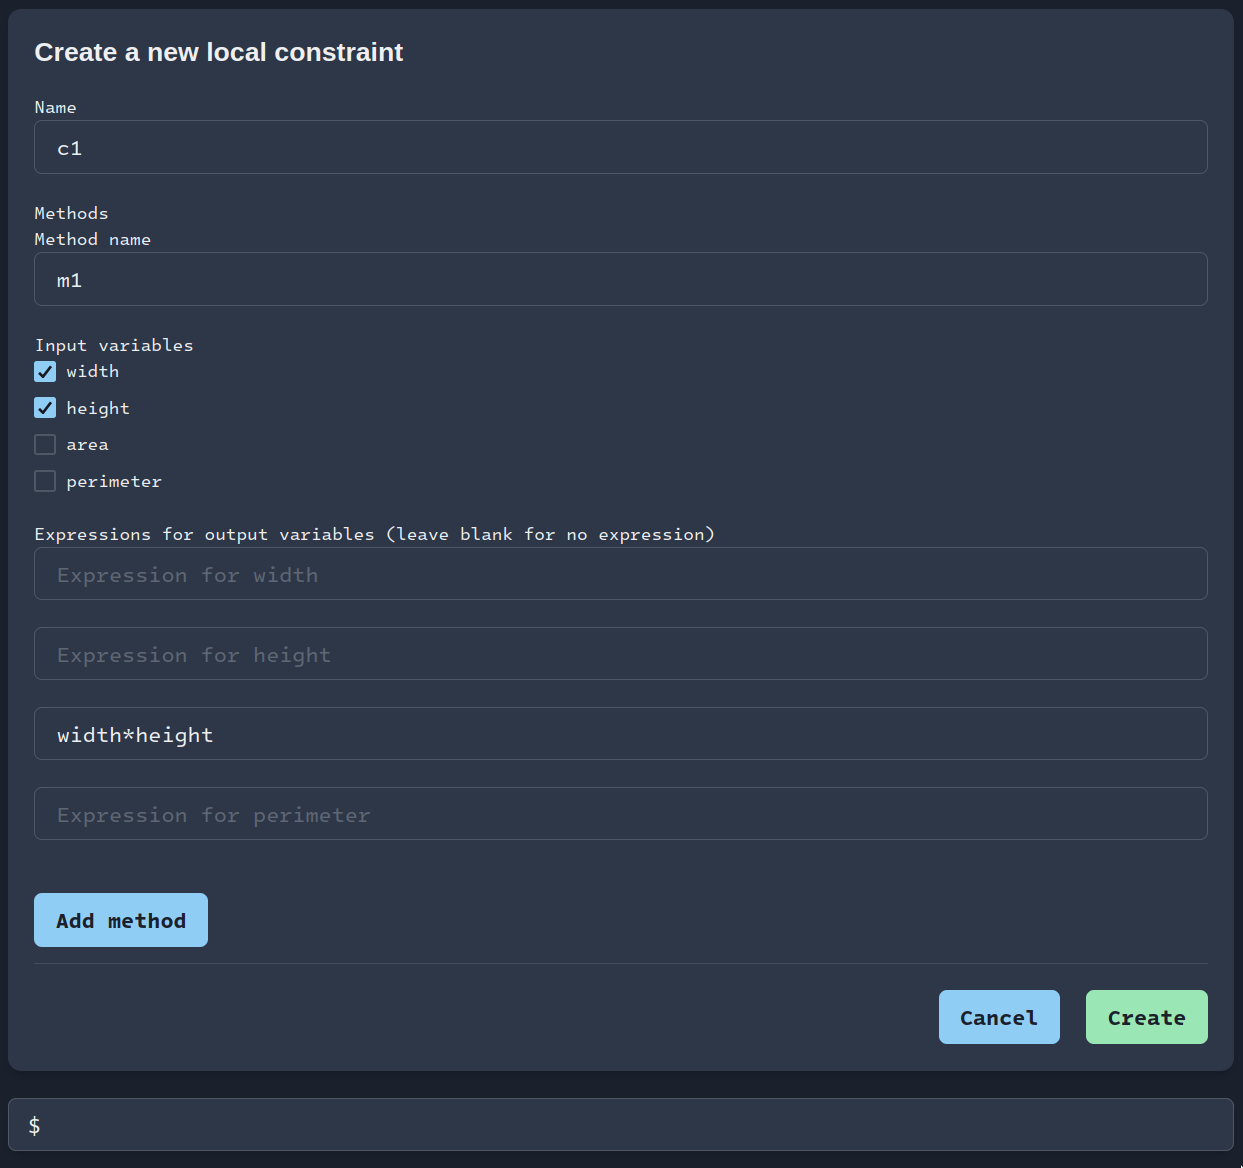
\includegraphics[width=\textwidth]{figures/dialog.png}
  \caption{The constraint dialog.}
  \label{fig:dialog}
\end{figure}

\subsection{Project Structure}
\label{sec:projectstructure}
The project\footnote{Found at \url{https://github.com/boaanes/319}} is structured in two parts, the frontend Web-CLI (found in the directory \texttt{web-cli}) as a React project, and the backend Haskell API (found in the directory \texttt{server}) as a Stack project.

To run the entire application locally, a user can either use Stack\footnote{\url{https://docs.haskellstack.org/en/stable/}} and Yarn\footnote{\url{https://yarnpkg.com/}}, or Docker\footnote{\url{https://www.docker.com/}}.

To run using Stack and Yarn, open two terminals, one in the \texttt{web-cli} directory and one in the \texttt{server} directory. In the \texttt{web-cli} directory, run the command \texttt{yarn start}, and in the \texttt{server} directory, run the command \texttt{stack run}. This will start the frontend and backend respectively, and the frontend application can be accessed at \url{http://localhost:3000}.

To run the entire application using docker, Docker must be installed. This repository can either be cloned and run using \textit{docker compose}\footnote{\url{https://docs.docker.com/compose/}} by running the command \texttt{docker compose up} in the root directory. The frontend application will then be available at \url{http://localhost}

The easiest and simplest solution to runnig the application however, is to use the Docker images for both the frontend and backend hosted at Docker Hub\footnote{\url{https://hub.docker.com/}}. By running the application this way, the only 
prerequisite is to have Docker installed, as there is no need to clone the repository. This can be achieved by running the following commands in sequence:

\begin{lstlisting}[language=bash]
docker run --name haskell-server -p 8000:8000 -d boaanes/319-haskell-server
\end{lstlisting}

\begin{lstlisting}[language=bash]
docker run --name react-app --link haskell-server:haskell-server -p 80:80 -d boaanes/319-react-app
\end{lstlisting}

In addition to the directories for the application itself, there is a directory \texttt{report} containing the \LaTeX{} source code for this report, as well as additional resources (such as figuers and generators) used in this report.

\section{Conclusion}
\label{sec:conclusion}
In this report we have presented a tool for visualizing constraint systems. The tool is designed to be used by anyone who want to experiment with MDCSs and structure manipulation of lists. It is intended to be used as a tool for debugging and understanding constraint systems in general. The tool is implemented as a web application, with a Haskell backend and a React frontend, and is designed to be used entirely through the terminal, where the user can interact with the application by issuing commands.

In addition to this, the application itself is fit for demoing MDCS to students, as it should be farily easy to use and understand. Features such as highlighting variables and constraints also help in this context of teaching. 

\clearpage
\bibliographystyle{plain}
\bibliography{generators/refs}

\end{document}
